\documentclass[twoside,letterpaper]{sig-alternate}
\usepackage[margin=1in]{geometry}
\usepackage[utf8]{inputenc}
\usepackage{url}
\usepackage{eurosym}
\usepackage{tikz}
%\usepackage{listings}
%\usepackage{graphicx}
%\usepackage{wrapfig}
%\usepackage{caption}
%\usepackage{subcaption}

\usetikzlibrary{cd}
\usetikzlibrary{shapes,arrows}
\usetikzlibrary{positioning}
\usetikzlibrary{calc}

\def\mathcomma{,}
\def\mathperiod{.}

\def\mathcomma{}
\def\mathperiod{}

\title{First Contact with Identity-based encryption}
% \subtitle{}
\author{Jeffrey Burdges, Florian Dold, Christian Grothoff, Neal Walfield}
\date{\today}

\begin{document}
\maketitle


\begin{abstract}
We argue that a limited use of identity-base encryption would improve
the security of trust-on-first-use key establishment protocols without
negative consequences on information leakage or usability.
\end{abstract}


\section{Introduction}

Usable key management is the central problem for widespread use
of encryption.

Highly secure decentralized solutions like the Web-of-Trust~\cite{wot}
leak social graph data since the key signing graph is public and key
lookups use a handful of key servers.  The GNU Name System provides a
model resembling the web-of-trust that leaks less profusely, but
offers no protection against confirmation attacks~\cite{gns}.  Both
of these schemes face significant deployment and adoption challenges.

Several recent proposals~\cite{openpgp-tofu,pep} address the
deployment and usability issues of the Web-of-Trust using
trust-on-first-use (TOFU).  Here, the endpoints hope that their first
interaction was not modified by a man-in-the-middle adversary, and
henceforth use the keys exchanged on first contact.

\section{Our Design}

We propose to strengthen TOFU by using a trusted third party (TTP)
that assists authentication.  The TTP would provide an authentication
service using identity-based encryption (IBE)~\cite{ibe}.  The
authentication service allows the owner of an e-mail account to
obtain a private key from the service (via e-mail).  The IBE scheme
then allows anyone who has the public key of the authority to derive
the corresponding public key, without ever contacting the authority.
This authority-derived key pair would then be used to secure the
first contact.

During the first contact, the parties would, as before, exchange
public keys based on locally generated non-IBE key material.  This
way, the scheme strictly strengthens TOFU by offering encryption
and authentication for the first contact.  If the authority has been
compromised, or if the communication channel over which the user
obtained the private key from the authority is monitored, the scheme
reverts back to the security of TOFU.

\begin{figure}[h]
\centering
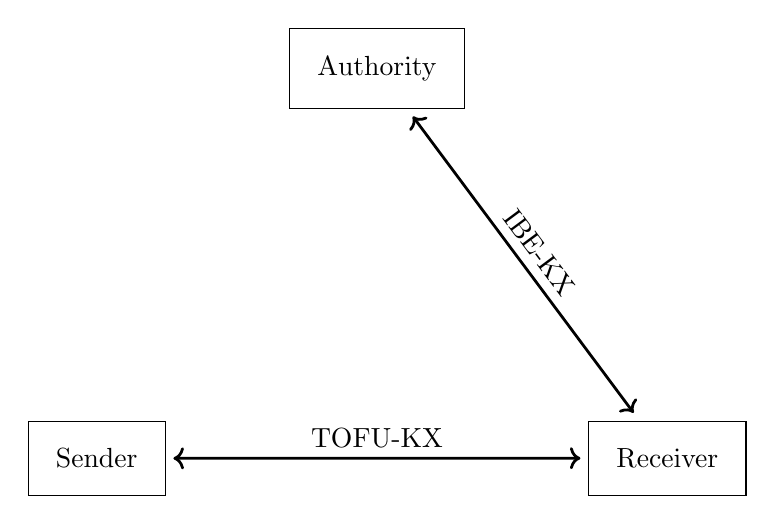
\begin{tikzpicture}
 \tikzstyle{def} = [node distance= 5em and 7em, inner sep=1em, outer sep=.3em];
 \node (origin) at (0,0) {};
 \node (authority) [def,above=of origin,draw]{Authority};
 \node (sender) [def, draw, below left=of origin] {Sender};
 \node (receiver) [def, draw, below right=of origin] {Receiver};

 \tikzstyle{C} = [color=black, line width=1pt]

 \draw [<->, C] (authority) -- (receiver) node [midway, above, sloped] (TextNode) {IBE-KX};
 \draw [<->, C] (sender) -- (receiver) node [midway, above, sloped] (TextNode) {TOFU-KX};
\end{tikzpicture}
\caption{Architecture overview.}
\label{fig:arch}
\end{figure}

Figure~\ref{fig:arch} shows the interactions in the proposed design.
With just TOFU, the adversary has to compromise the first contact
between sender and receiver.  With the addition of an authority
providing additional IBE-based key material, the adversary has to {\em
  additionally} compromise the link between authority and receiver.

Securing the link between authority and receiver against a passive
adversary is generally easy, as the key request itself can be
encrypted using a well-known public key of the authority, and can
include a public key of the receiver. This way, the authority's
response containing the private (IBE) key can already be encrypted.
However, this does not help against an active adversary who controls
the link can initiate requests.


The use of multiple authorities can further strengthen the design.
This forces the adversary to actively compromise all paths between all
authorities and the receiver.  Given multiple authorities, the sender
can freely pick which authorities she trusts (to secure first
contact); given any such subset the receiver can then simply request
the missing key material.


\section{Key Rotation}

We observe that one principle weakness of our proposal is that
identity-based keys are not ephemeral.

If, for example, an e-mail address is assigned to a different user,
the IBE-generated private key remains the same.  While this could
even be desireable for functional e-mail addresses, sometimes key
rotation may be preferred.

A simple solution is for the authorities to rotate their keys. This
will require new public keys to be distributed to all senders.
Distributing this key material to senders could be done in a way
similar to how operating systems distribute root keys for X.509
CAs, ensuring that users rarely have to manually intervene.


\section{Why Identity-based Encryption?}

The use of IBE is critical in our design, as it allows the sender to
{\em compute} the public key of the receiver without interacting with
anyone.  Asking about key material would be problematic, as the sender
obtaining public keys from a TTP---or equivalently from key servers in
the Web-of-Trust---unduely leaks meta-data about user's social graph,
which can be harmful to life and limb~\cite{skynet}.  Furthermore,
such interactions tend to not work well with the SMTP protocol.

There have been various proposals for the use of TTPs to certify keys,
such as certificate authorities (CAs) in X.509 or the more recently
created certificate transparency~\cite{certtrans} monitoring
framework.  However, these schemes expect that certificates are
provided by the recipient to the sender during the TLS
handshake~\cite{tls}.  Such a method does not interoperate well with
SMTP, which operates asynchronously without a bidirectional
communication channel between sender and recipient.


\section{Practical considerations}

The receiver has to contact the authority to obtain his private
key, and the authority must send the private key via e-mail to
the receiver as the verification step is simply that the receiver
has control over the e-mail account.  This requires that the
e-mail client is extended with the ability to request key material.

Requesting key material becomes a bit tricky if the encryption tool is
separate from the e-mail client.  For example, GnuPG does not directly
interact with SMTP, and it will require a non-trivial architectural
evolution to support requesting such private keys on-demand.


\section{Security implications}

We employ IBE {\em only} for the weak form of authentication provided
by the trusted authentication server, while full authentication still
requires that users verify fingerprints.  Our method also does not
keep users from establishing strong keys out-of-band or via the
Web-of-Trust.  This is crucial, as IBE fundamentally supports key
escrow, so we have to assume that certain adversaries will be able to
obtain the IBE key material.

Hence, a major danger in the design is the psychological effect, as
users may skip fingerprint verification due to an overreliance on the
low level of additional security provided by the authorities.  It is
thus important to point out that our scheme remains fundamentally
vulnerable to an attacker who can both extract the recipient's private
key from the authority, and attack the transport during the initial
exchange.


\section{Conclusions}

We have proposed a scheme to strengthen TOFU-based key discovery using
authorities that generate private keys using identity-based
encryption.  The scheme has the advantage that it works within the
asynchronous model of OpenPGP and does not leak meta data to the
authority.  However, it would require tight integration of the
decryption engine with the SMTP client.


\section*{Acknowledgements}

This work benefits from the financial support of the Brittany Region
(ARED 9178) and a grant from the Renewable Freedom Foundation.


%\newpage

\bibliographystyle{abbrv}
\bibliography{msg,ecc,ibe}

\end{document}


\section{}
